\documentclass{tufte-handout}
\usepackage{amsmath}
\usepackage{pdfpages}
\pagestyle{empty}
\usepackage[utf8]{inputenc}
\usepackage{mathpazo}
\usepackage{microtype}

\usepackage{tikz}
\usetikzlibrary{matrix}
\usetikzlibrary{chains}
\usetikzlibrary{decorations}

\title{Flow behind enemy lines}
\author{Thore Husfeldt}

\begin{document}

\maketitle

\subsection{Description}
Find a maximum flow and the corresponding minimum cut in a flow network that describes the railway system of the Eastern Bloc during the Cold War.

We're behind on the five year plan!
The party secretary from Minsk has been tasked with reducing the capacity of one or two railway lines by 10 or 20 kilotons per day.
Luckily, you have acquired data about the full Soviet railway system from an American double agent.

\subsection{Requirements}

Your algorithm successfully computes a maximum flow and a minimum cut on the Americans' data.

Moreover, you can use it to study the situation when you reduce the capacities on the lines from division 4W to divisions 48 and 49.
Analyze the effects of reducing their capacities  to 10 or 20 (on either or both).

\subsection{Deliverables}

\begin{enumerate}
  \item The source code for your implementation
  \item A report in PDF.
  Use the report skeleton in the {\tt doc} directory.
  \end{enumerate}

\subsection{Sources}

The image on the next pages shows the Soviet railway network from T. E. Harris, F. S. Ross, ``Fundamentals of a Method for Evaluating Rail Net Capacities'', US Air Force Project RAND research memorandum RM–1573, October 24, 1955, declassified on 13 May 1999. You can find the original document on the net.
Cool stuff.
Print it and leave it on your desk, to impress friends and family.

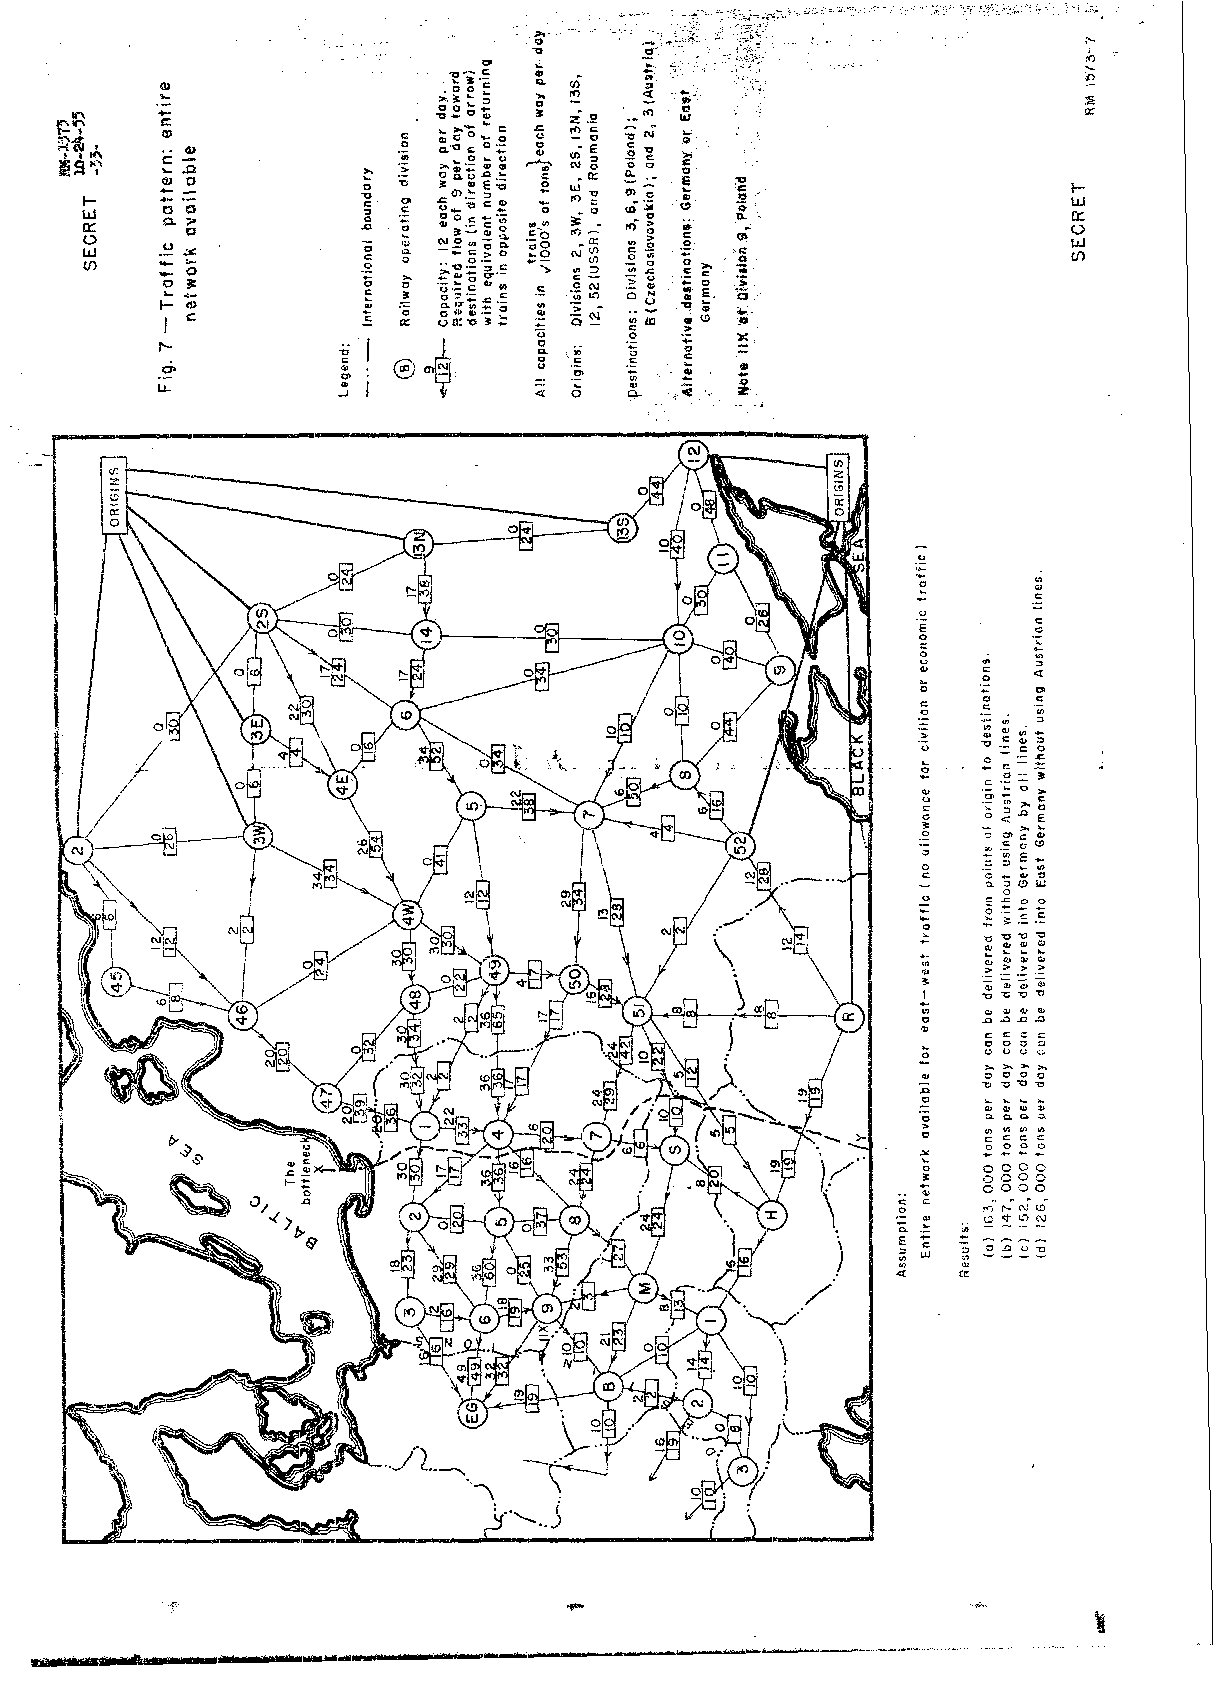
\includepdf{secret.pdf}

\end{document}
